\section{\vt\ Usage Study}
\label{sec:label}

In this section, we present the empirical study on how 
academic people use \vt. 
We will first discuss how we collect academic papers to conduct the study, 
and then we will present our findings and implications. 

\subsection{Methodology}

We leverage published academic papers to understand 
how academic people use \vt,
since published papers usually contain detailed descriptions 
about how the authors use \vt\ in their projects, if \vt\ is involved. 

To collect academic papers, we search for keyword ``\vt'' in Google Scholar. 
In total, we find 101 conference papers published in the last ten years.
We then manually inspect descriptions related to \vt\ in these papers. 
For 87 papers, the authors either use \vt\ 
to build a data set for their evaluation~\cite{ford2009analyzing,android-1,email-vt-1,kharraz2016unveil} 
or leverage querying \vt\ as one building block of their
techniques~\cite{vt-component-1,vt-component-2,vt-component-3}. 
These 87 papers are targets of our \vt{} usage study. 
For the left 14 papers, their authors just discuss \vt\ as a part 
of technical background~\cite{not-use-1,bayer2009scalable,jiang2012dissecting}, and 
they do not use \vt\ in building their techniques or evaluation. 
Therefore, we ignore these papers in our study. 


\begin{figure}%
\centering
\subfigure[Conference]{%
\label{fig:conference}%
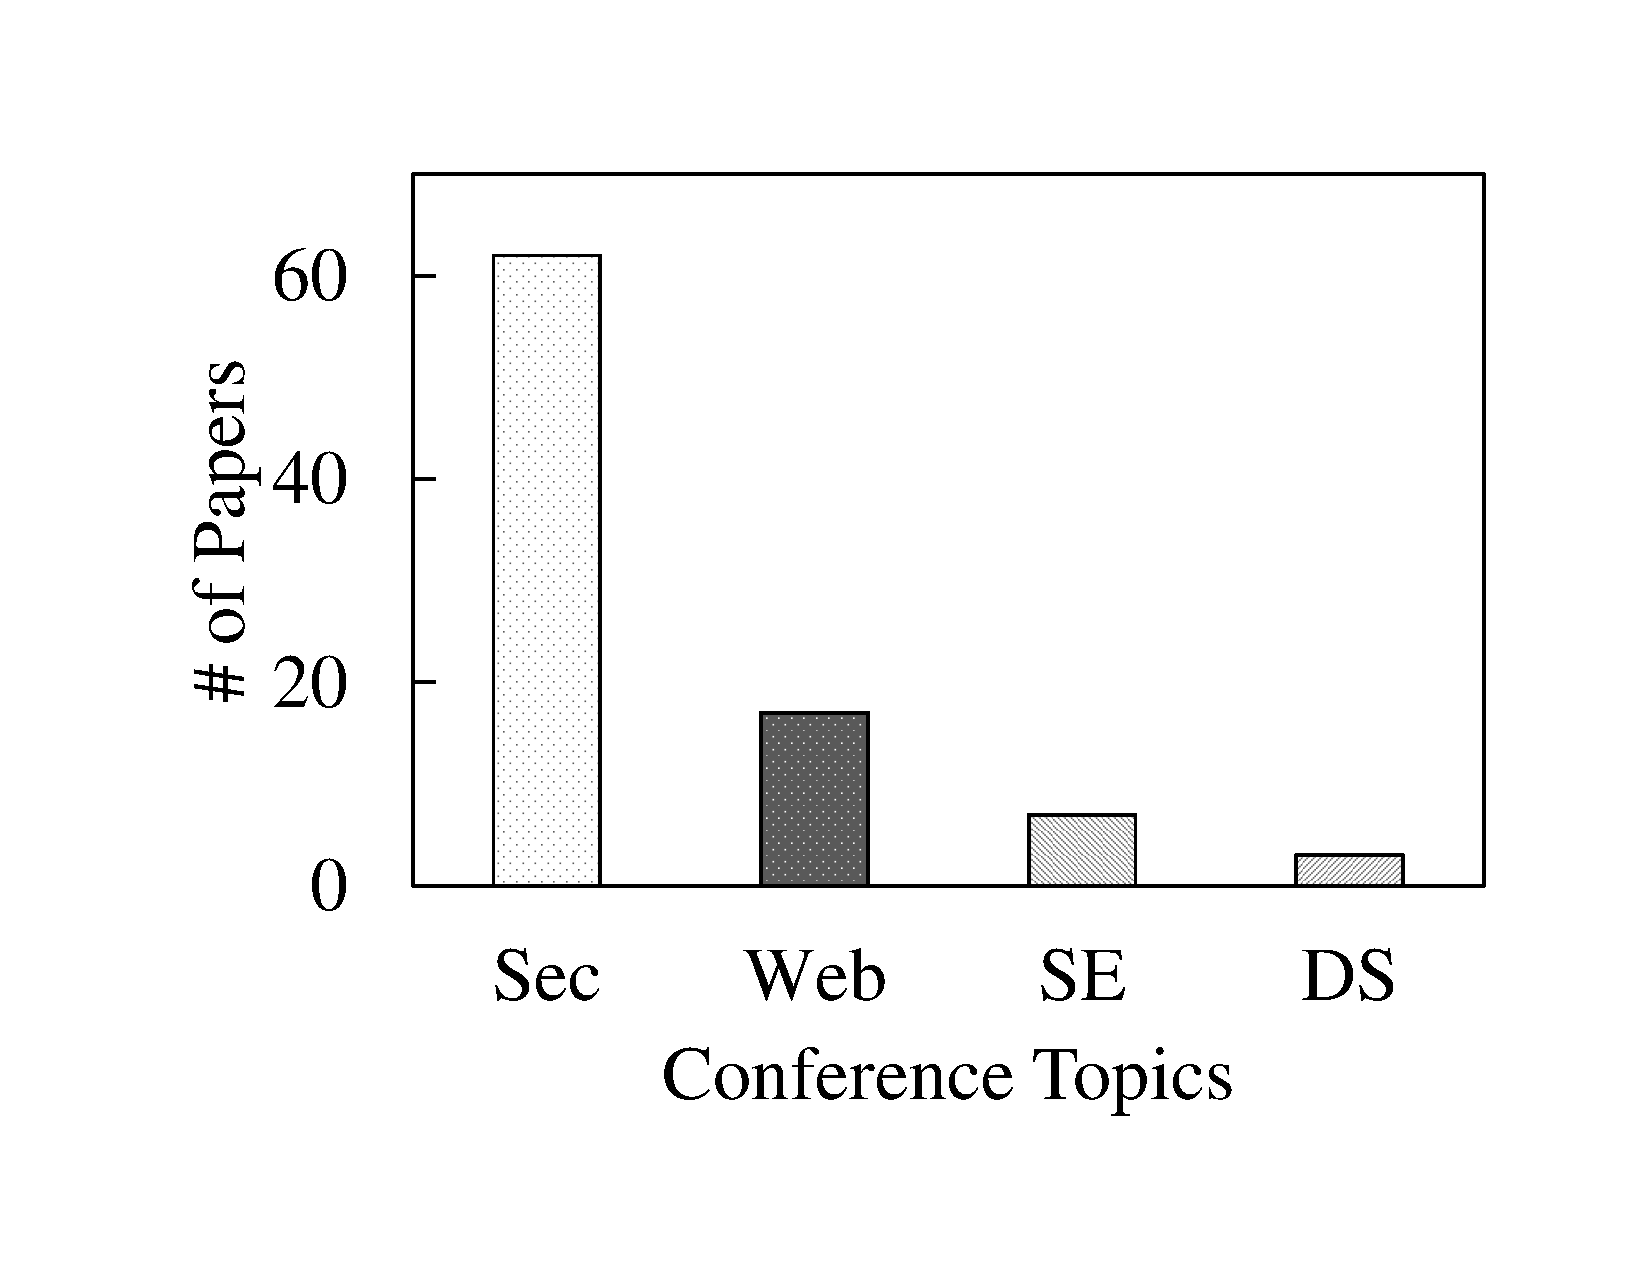
\includegraphics[width=1.45in]{figure/literature-confs}}%
\qquad
\subfigure[Publication Year]{%
\label{fig:year}%
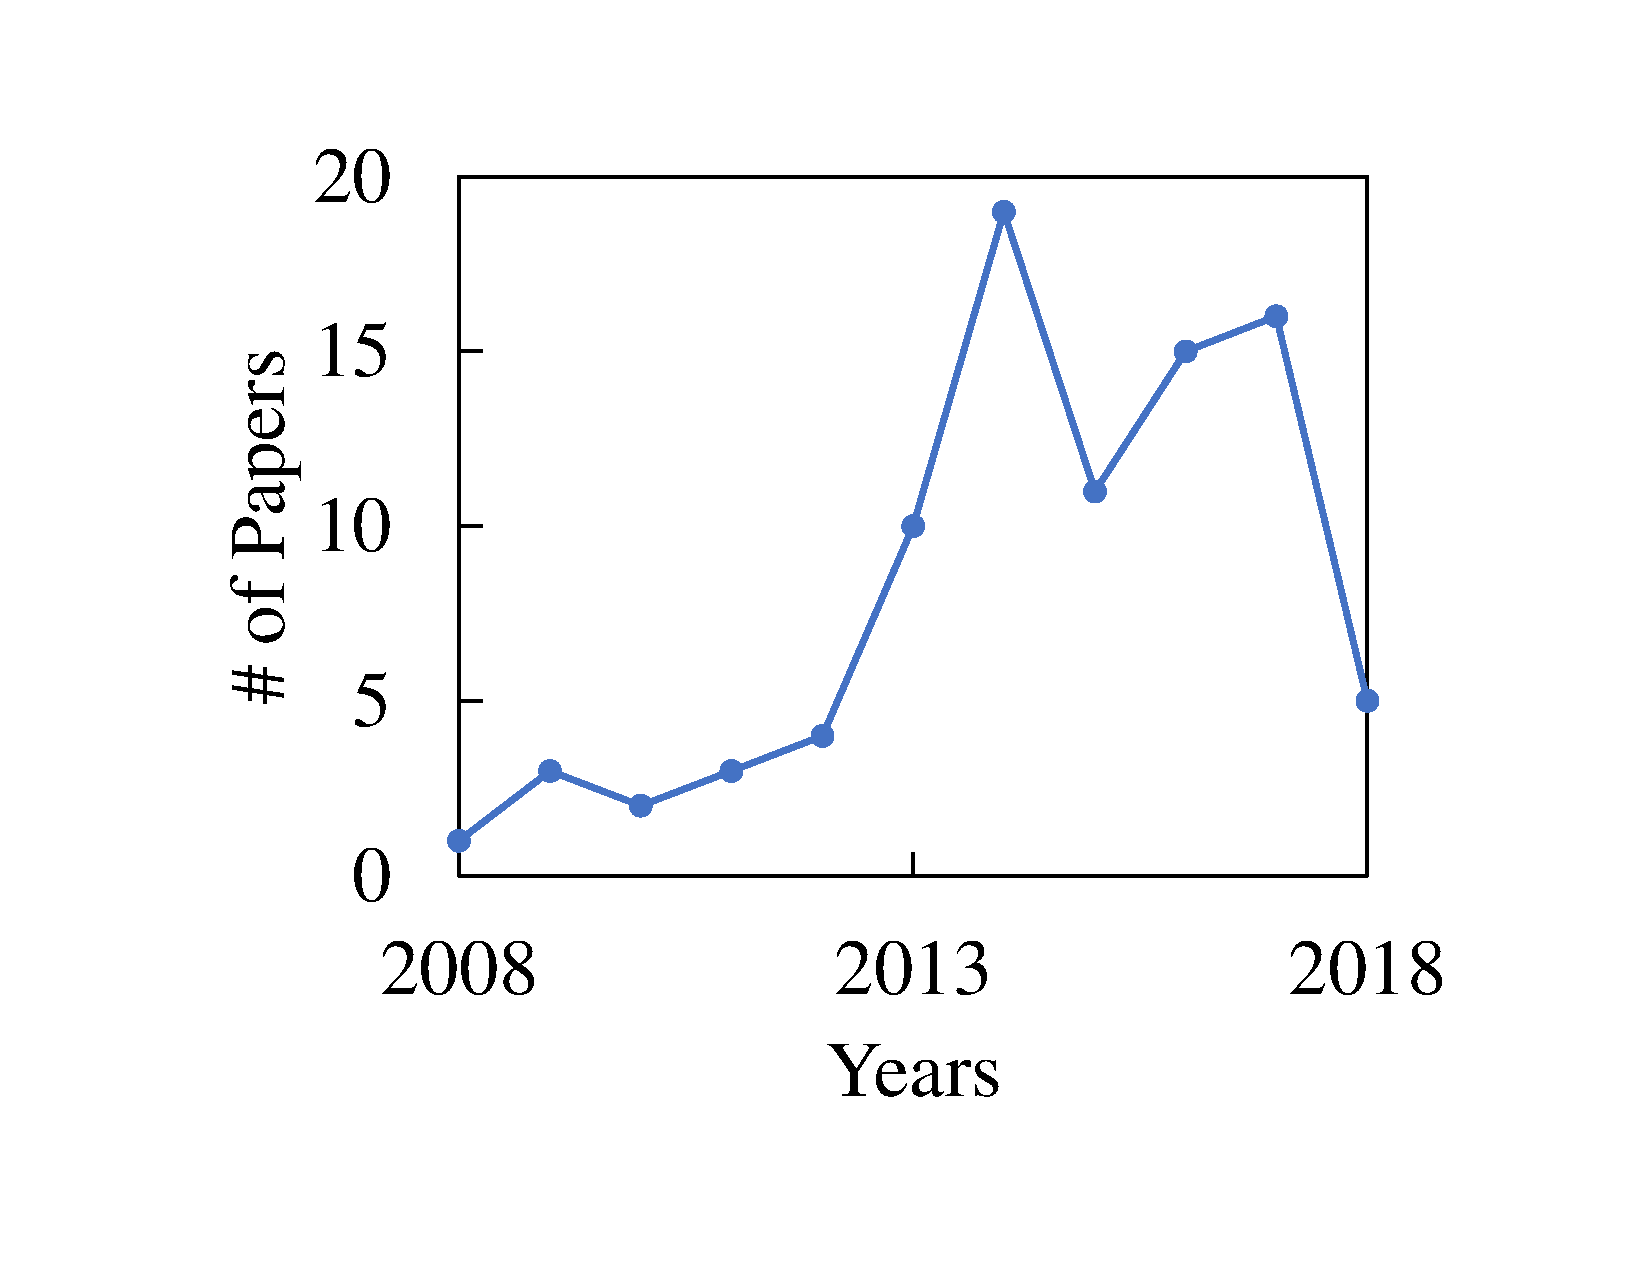
\includegraphics[width=1.45in]{figure/literature-years}}%
\mycaption{fig:char}
{Characteristics of our studied papers.}
{Sec: Security, DS: Data Science and SE: Software Engineering.}
\end{figure}




As shown in Figure~\ref{fig:conference}, 
our collected papers mainly come from famous academic conferences 
in four research areas, security, software engineering, data science, and web. 
For example, in total, we study 62 papers published in security conferences,
and 28 of them come from the top four security conferences, 
IEEE S\&P, CCS, Usenix Security, and NDSS.
As shown in Figure~\ref{fig:year}, 
we have at least one studied papers 
published in each year from 2008 to 2018. 
19 studied papers are published in 2014, 
and it is the year with largest number. 
Our studied papers cover different types of malware, 
such as Android APK~\cite{android-1,arp2014drebin,huangvt2016bigdata}, 
Portable Executable (PE) files~\cite{bayer2009scalable,pe-vt-1,pe-vt-2}, 
Flash~\cite{ford2009analyzing,wressnegger2017looking}, 
PDF~\cite{pdf-vt-1,carmony2016extract}, and so on. 
To sum up, we believe our studied paper is a representative data set 
to understand how academic people use \vt{}. 

\subsection{Findings and Implications}
We mainly want to answer two questions through our study.
First, \vt{} applies multiple antivirus engines to scan every submitted file 
and returns all detection results to user.
Different engines may disagree with each other.
We want to figure out how academic users aggregate results from different vendors 
and make the decision about whether a submitted file is benign for malicious. 
Second, \vt{} keeps updating antivirus engines. 
Intuitively, detection results could change when the same file is submitted twice.
We want to know whether or not academic users consider 
possible result changes on \vt{} over time.   


\noindent{\underline{How detection results are merged?}}
For 72 out of 89 (80.89\%) studied papers, 
their authors leverage a threshold to decide whether a submitted file is 
malicious or not. 
The threshold can either be a absolute number, 
or a ratio of the number of engines with malicious labels over all engines.
There are 26 studied papers, 
whose authors consider a submission is malicious, 
if any engine labels it as malware. 
For another {\color{red} XXX} papers, their authors 
use a absolute threshold number that is larger than one. 
Authors of {\color{red} XXX} papers use a ratio as their threshold.  
For the left 17 papers, their descriptions about how to merge \vt{} results 
are not clear enough for us to study. 

Since academic users widely use a threshold 
to decide a submitted file is malicious or not, 
we want to understand how the threshold is counted or calculated. 
Specifically, we want to know whether every engine 
on \vt{} is counted in the same way, or they have different weights.   
In most cases (64/72), the paper authors treat each engine equally.
For the other 8 papers, the authors think that different engines 
may have different reputations, 
and they only consider a small set of engines with 
good reputation.
For example, \citet{five-vendors-1} only consider five vendors' results, 
while \citet{arp2014drebin} only inspect results from ten vendors. 

\noindent{\underline{\bf{Observation 1:}}}
{\it{
Academic users usually use threshold to interpret detection results from \vt{}, 
and they mainly treat different vendors equally during the calculation of the threshold value, 
without considering possible difference across vendors.  
}}


\noindent{\underline{Whether possible changes are considered?}}
When a new malware sample is developed, 
it is likely that very few engines can detect it. 
It takes vendors some time to reverse engineer the sample.
Intuitively, there will be more and more engines 
that can detect the sample as time goes on. 
Therefore, we anticipate that when the same file 
is submitted to \vt{} more than once,
the detection results could change. 
However, we find that only three papers in our paper set
consider the evolution of engines and possible 
changes of detection results on \vt{}. 
For example, \citet{neeles} only consider files submitted to \vt{} 
several months ago to make sure that their collected samples 
are correctly classified by \vt{} vendors. 
\citet{wressnegger2017looking} submit the same samples multiple 
times to identify samples that were previously missed by \vt{} engines.  

\noindent{\underline{\bf{Observation 2:}}}
{\it{
Academic users seldom consider possible 
result changes of anti-virus engines on \vt{}, 
and they usually rely on analysis results from only \vt{} scanning. 
}}

\noindent{\underline{Discussion.}}
We find that academic people use \vt{} mainly under two assumptions.
First, detection results from different engines have the same quality,
so that results from different engines are treated equally. 
Second, although detection results on \vt{} could change over time, 
the chances do not widely exist and only have very limited impact. 
However, these two assumptions may not be correct. 
In the following sections, we will design experiments and 
systematically evaluate whether or not these two assumptions are correct. 

\noindent{\underline{\bf{Implication 1:}}}
{\it{
When \vt{} is used in academic papers, the papers' results must be 
interpret together with how \vt{} is used. 
}}

